%!TEX root = ../konzept.tex

\section{Problemstellung}
Reisende, die während ihres Aufenthalts an mehreren Orten Halt machen, werden oftmals vor dem Problem gestellt, eine geeignete Unterkunft für die Nacht zu finden. Vorhandene Systeme ermöglichen bereits eine zufriedenstellende Suche von Alternativen und gewährleisten eine Übersicht eingetragener Hostels, Campingplätze oder Hotels. Im Gegenzug dafür, fordern sie jedoch vom Reisenden viele Gegenleistungen, die ihn in seiner Flexibilität und Reisefreiheit einschränken.\\
Wesentliche Punkte die bei dieser „herkömmlichen Art des Reisens“ beachtet werden müssen sind folgende:
\begin{itemize}
   \item \textbf{Frühzeitige Planung}: Gerade wenn man einen Urlaub während der Hochsaison plant, ist es notwendig bereits im Vorfeld für entsprechende Reservierungen zu sorgen. Alternativ wird man vor noch höheren Kosten gestellt oder findet keine gewünschte Unterkunft. 
   \item \textbf{Geringe Flexibilität}: Eingegangene Reservierungen sind weitestgehend verbindlich. Die Reiseplanung wird damit festgesetzt und ermöglicht keine kurzfristigere Änderung. Spontanität, Variation der Reiseroute und Zeitplan sind damit nicht möglich oder mit aufzuwendende Kosten verbunden. 
   \item \textbf{Kosten}: Gängige Unterkünfte stellen eine sichere Option dar, sind für viele Reisende jedoch ein hoher Kostenfaktor. Dieser kann sowohl Einfluss auf die Reisedauer als auch den Reiseort haben. Oftmals wird dabei auf ein günstigeren Kompromiss eingegangen. 
\end{itemize}

Diese Punkte berufen sich dabei auf eigene Erfahrungen und den Schwerpunkten, die eine Reiseplanung notwendigerweise mit sich führen. Alle drei Aspekte stehen dabei auch in einem gewissen Zusammenhang, so dass  Auswirkungen auf einzelne Faktoren die Restlichen beeinflussen. Von Seiten des Marktes, wird der Reisende zudem stark davon aufgefordert auf diese einzugehen, indem mit einem Frühbucherrabatt geworben wird, der dem Kunden deutliche finanzielle Vorteile bietet\footnote{ http://www.drv.de/presse/presseinformationen.html Artikel Frühbucher sind im Vorteil}.\\    

Mit der Motivation des Reisenden, ergibt sich innerhalb des Konzeptes auch eine zweite Kernzielgruppe des 
Systems. Da die Mieter auf eine alternative Unterkunft ausweichen, gibt es bei jeder Aktivität einen Vermieter 
als Gegenpart. Find your Camp soll beide Kommunikationsseiten betrachten und beide gleichermaßen in der 
Umsetzung ihrer Aufgaben unterstützen. Der zuvor angesprochene Frühbucherrabatt, ist dabei nicht ledigliche 
eine gutmütige Geste des Anbieters, sondern er sichert sich damit Kunden und kalkulierbare Einnahmen. Er 
profitiert dementsprechend von diesem Angebot.\\
Sollen die Problempunkte des Reisenden verringert werden, so hat dies auch Einfluss auf die Vermieterseite. Zu 
nennen wäre hierbei, dass er nicht mit festen Besucherzeiten rechnen kann und in seinem Angebot sehr flexibel 
sein muss. Gerade für öffentliche Anbieter, die von den Einnahmen ihr Geschäft betreiben ist das ein kritischer
Faktor. In Anbetracht des Projektes, ist dieser Trade-Off weiterhin mit diesen Folgen verbunden, stellt aber 
keine Existenzgefahr der Anbieter dar, weil sie grundsätzlich nicht mit festen Kunden zur Hochsaison rechnen 
können. Dennoch setzt das voraus, dass die Anbieter auf Anfragen deutlich kurzfristiger und unorganisierter 
reagieren müssen.
Bezogen auf die Problemdomäne, ergeben sich für Leute die als private Vermieter agieren wollen, folgende Probleme in der jetzigen Situation. Einige der Ansätze ergaben sich auch in Zusammenhang mit der durchgeführten Marktanalyse, die im folgenden Kapitel genauer beschrieben wird.
\begin{itemize}
   \item \textbf{Sicherheit der Daten}: Vorhandene Portale setzen darauf, dass der Anbieter seine Informationen
auf dem Server speichert und bereits bei der Suche des Mieters einsehbar sind. Dadurch werden sensible Daten
für viele Leute transparent und können zum Missbrauch führen\footnote{Beispiel Campinmygarden}. 
   (Dieser Schwerpunkt soll im geplanten System durch die Verteiltheit geregelt werden (Kapitel 4.2))

   \item \textbf{Anfragen sind nicht immer relevant}: Der Mietende schreibt in bisherigen Beispielen mehrere potentielle Vermieter aufgrund eines Inserates an. Dabei werden alle Optionen angezeigt die vorhanden sind. Speziell für den Vermieter, ergeben sich damit auch Anfragen, die aufgrund diverser Faktoren nicht wahrgenommen werden können. Durch die Allokation des Systems, soll die Kommunikation auf relevante Anfragen hin gefiltert werden und das Usermatching vom System aus organsieren. (Kapitel 4.1)
\end{itemize}


In den vergangenen Jahren entwickelte sich, neben etablierten Unterkünften, die den Besucher vor genannte Probleme stellen, ein Trend der sich auf das Konzept der Shared Economy beruft.\\
Share Economy ist ein Begriff, der durch den Wirtschaftswissenschaftler Martin Weitzman geprägt wurde und sagt aus, dass sich der Wohlstand aller erhöhen wird, je mehr unter den Marktteilnehmern geteilt wird\footnote{Publiziert in The Share Economy: Conquering Stagflation, Harvard University Press, 1984 \\http://scholar.harvard.edu/weitzman/publications/share-economy}. Auf die zugrunde liegende Anwenderdomäne bezogen bedeutet dies, das Teilen von vorhandenen Grundstücken an Reisende. Der Anbieter verleiht ein Teil seines Eigentums und zieht daraus einen zusätzlichen Nutzen, den er unter gewöhnlichen Umständen nicht erhält. Er baut sozialen Kontakt auf und teilt seine ungenutze Ressourcen zum Vorteil aller Beteiligten, indem er für sich Einnahmen erzielt (damit eventuell auch vorhandene Unkosten beseitigt, die durch Besitz auftreten) und für den Mieter ein lokratives Angebot bietet. Der Grundsatz liegt prinzipiell aber nicht darin, seinen Besitz zu vergrößern, sondern im Sinne aller Beteiligten Vorteile zu schaffen. Daher ist auch keine Verleihgebühr des Vermieters notwendig, wenn er einfach die soziale Motivation und Erfahrung als Gewinn erachtet. Während des Leihprozess, sollte sich für ihn jedoch keine nachhaltigen Negativfolgen ergeben, wie Unbrauchbarkeit des Grundstückes. \\  


Beispielsweise am Couchsurfing\footnote{www.couchsurfing.org} zeigt sich, dass es eine Nachfrage an alternativen Unterkünften gibt und dieser Anwendungsbereich bereits mehr als nur ein erster Versuch ist. Der Zuspruch liegt grundsätzlich auf sozialen Aspekten sowie dem Kostenfaktor begründet und hat sich zeither in mehr als 100 000 Städten weltweit platziert. 2004 gegründet, entwickelte sich bis ins Jahr 2011 eine große Anwenderschafft, die auch 2013 noch, nach fast 10 Jahre, an Zuwachs gewinnt. 
\newpage
Folgende Grafik (Abb.\ref{Couchsurfer}), zeigt die Verteilung der teilnehmenden Anwender im Jahr 2011\footnote{Quelle http://upload.wikimedia.org/wikipedia/commons/6/6d/Couchsurfers\_by\_country.png}. 

\begin{figure}[H]
\centering
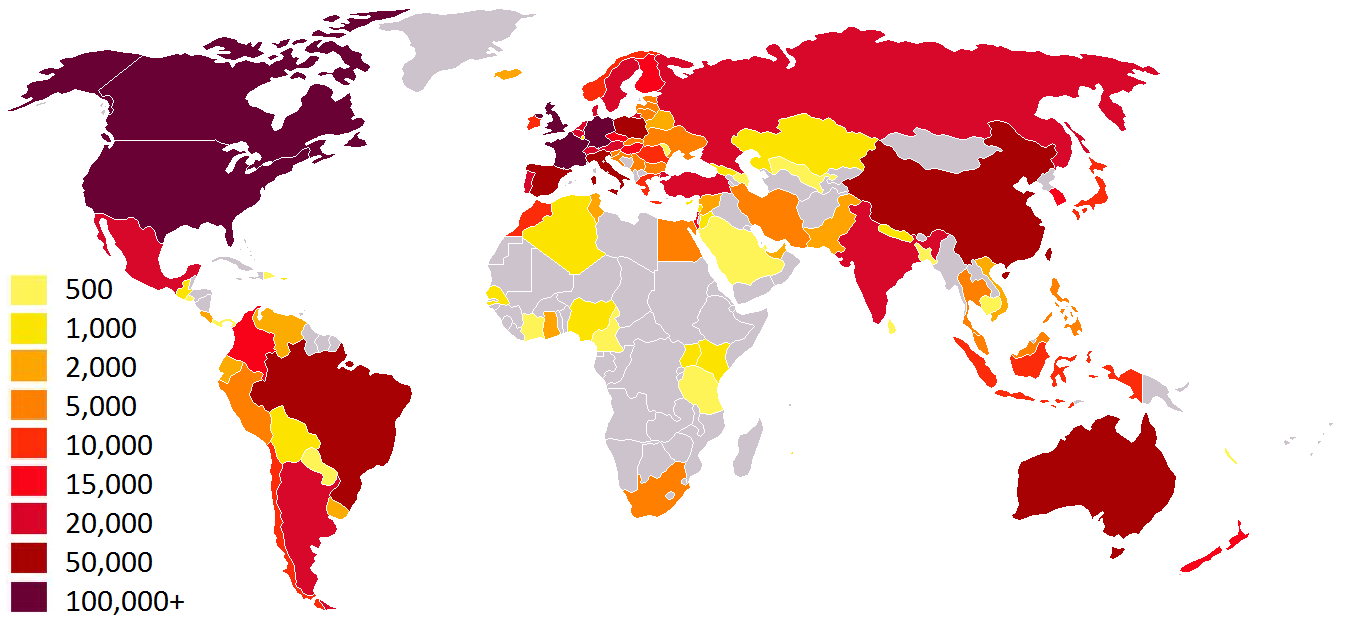
\includegraphics[width=1.0\textwidth]{./images/couchsurfers.png}
\caption{Länder 2011 mit mehr als 500 registrierten Usern} 
\label{Couchsurfer}
\end{figure}


Im Januar 2013 fasste die Seite 5.5 Millionen registrierte User.\footnote{Informationen über www.couchsurfing.org/n/about und http://en.wikipedia.org/wiki/CouchSurfing} Als weiteres relevantes Beispiel wäre Airbnb\footnote{Webpräsenz www.airbnb.de} zu nennen, die einen ähnlichen Ansatz verfolgen, bei dem private Anbieter Unterkünfte zur Verfügung stellen, dabei jedoch eine entsprechende finanzielle Gegenleistung einfordern.
Das 2008 gegründete Unternehmen bietet derzeit über 500.000 eingetragene Inserate und zeigt, dass auch im bezahlten Place Sharing Bereich großes Interesse der Reisende vorhanden ist. Preislich spielt dieser Anbieter dabei sogar auf dem Niveau gängiger Anbieter.\\

Das Sharing Prinzip hat sich auch im Alltag durchgesetzt.
Car Sharing, Bike Sharing oder Carspace Sharing, sind populäre Umsetzungen und bereits in vielen Städten vorzufinden. Zahlreiche Studien zeigen, dass Sharing Economy ein wichtiger Aspekt der zukünftigen Wirtschaft sein wird und die Menschen bereit sind nach ihren Regeln zu handeln\footnote{Beispiel http://de.scribd.com/doc/38788695/The-New-Sharing-Economy-Study-Report-by-Latitude-and-Shareable-Magazine}.\\


 





  










%\newpage
%\subsection{Weiterführende Statistik}
%\textcolor{red}{Hier nochmal überlegen, ob die Inhalte dieses Unterpunktes wirklich relevant sind und zeitlich Akzeptabel.}\\


%Mit der einsetzenden Finanzkrise 2007, zeigte sich im Tourismus eine Entwicklung, die sich nicht nur auf Deutschland, sondern den gesamten Europäischen Raum abzeichnen lässt. 
%In folge der Krise handelten viele Urlauber, indem sie neue Möglichkeiten suchten ihre Übernachtungskosten zu reduzieren und wichen dabei auf öffentliche Campingplätze aus. 
%Zeitgleich konkurrieren vorallem asiatische Länder um die Gunst der Touristen, indem sie ein Billigsegment schaffen, dass viele Interessierte in ihre Gegenden zieht. Aufgrund der Steuerbelastung sowie Personalkosten etc. fällt es vielen europäischen Ländern schwer mit diesem Trend mitzuhalten.\\
%Als alternative gegenüber Hotelübernachtungen zeigen Statistiken, die von der European Commision erhoben und veröffentlicht wurden, eine Entwicklung der Campingplatzbesucher der letzten Jahre.  Während grundsätzlich in Skandinavien, sowie den Küsten und Bergregionen Europas großer Zuspruch herrscht, so lassen sich auch in Deutschland Gebiete identifizieren, die einen jährlichen Zuwachs von 10\% an Campingplatzbesucher gewinnen.\\

%Quelle: http://epp.eurostat.ec.europa.eu/statistics\_explained/index.php/Tourism\_statistics\_at\_regional\_level/de 
%Sichtdatum 20.10.2013




